% Adjust these for the path of the theme and its graphics, relative to this file
%\usepackage{beamerthemeFalmouthGamesAcademy}
\usepackage{../../beamerthemeFalmouthGamesAcademy}
\usepackage[utf8]{inputenc}
\usepackage{multimedia}
\graphicspath{ {../../} }

% Default language for code listings
\lstset{language=Python,
    keepspaces=true,
    breaklines=false
}

% For strikethrough effect
\usepackage[normalem]{ulem}
\usepackage{wasysym}

\usepackage{algpseudocode}

\usepackage{pdfpages}

\usepackage{circuitikz}

\iftoggle{printable}{
    \newcommand{\circuitcolour}{black}
}{ % else
    \newcommand{\circuitcolour}{white}
}

% http://www.texample.net/tikz/examples/state-machine/
\usetikzlibrary{arrows,automata}

\newcommand{\modulecode}{COMP260}\newcommand{\moduletitle}{Distributed Systems}\newcommand{\sessionnumber}{5}

\hypersetup{
pdftex,
pdftitle=\sessionnumber: Data Types,
pdfauthor=Ed Powley,
pdfdisplaydoctitle,
pdflang=en-GB
}
 
\begin{document}
\title{\sessionnumber: Data Types}
\subtitle{\modulecode: \moduletitle}

\frame{\titlepage} 

\part{Binary notation}
\frame{\partpage}

\begin{frame}
	\centering
	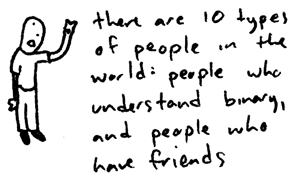
\includegraphics[width=0.7\textwidth]{10-types-of-people}
	\par\vspace{2ex}\par
	{\tiny Image credit: \url{http://www.toothpastefordinner.com}}
\end{frame}



\begin{frame}{How we write numbers}
	\begin{itemize}
		\pause\item We write numbers in \textbf{base~10}
		\pause\item We have 10 \textbf{digits}: $0, 1, 2, \dots, 8, 9$
		\pause\item When we write $6397$, we mean:
			\begin{itemize}
				\pause\item Six thousand, three hundred and ninety seven
				\pause\item (Six thousands) and (three hundreds) and (nine tens) and (seven)
				\pause\item $(6 \times 1000) + (3 \times 100) + (9 \times 10) + (7)$
				\pause\item $\left(6 \times 10^3\right)
				+ \left(3 \times 10^2\right)
				+ \left(9 \times 10^1\right)
				+ \left(7 \times 10^0\right)$
				\pause\item
				    \begin{tabular}{cccc}
				        Thousands & Hundreds & Tens & Units \\
				        6 & 3 & 9 & 7
				    \end{tabular}
			\end{itemize}
	\end{itemize}
\end{frame}

\begin{frame}{Binary}
	\begin{itemize}
		\pause\item Binary notation works the same, but is \textbf{base~2} instead of \textbf{base~10}
		\pause\item We have 2 \textbf{digits}: $0, 1$
		\pause\item When we write $10001011$ in binary, we mean: \par\pause
			$\phantom{+} \left(1 \times 2^7\right) + 
			\left(0 \times 2^6\right) + 
			\left(0 \times 2^5\right) + 
			\left(0 \times 2^4\right)$ \par
			$+ \left(1 \times 2^3\right) + 
			\left(0 \times 2^2\right) + 
			\left(1 \times 2^1\right) + 
			\left(1 \times 2^0\right)$ \par\pause
			$= 2^7 + 2^3 + 2^1 + 2^0$ \par\pause
			$= 128 + 8 + 2 + 1 \text{ (base 10)}$ \par\pause
			$= 139 \text{ (base 10)}$
	\end{itemize}
\end{frame}

\begin{frame}{Why binary?}
	\begin{itemize}
		\pause\item Modern computers are \textbf{digital}
		\pause\item Based on the flow of current in a circuit being either \textbf{on} or \textbf{off}
		\pause\item Hence it is natural to store and operate on numbers in base 2
		\pause\item The binary digits $0$ and $1$ correspond to \textbf{off} and \textbf{on} respectively
	\end{itemize}
\end{frame}

\begin{frame}{Converting to binary}
    \begin{center}
        \url{https://www.youtube.com/watch?v=OezK_zTyvAQ}
    \end{center}
\end{frame}

\begin{frame}{Bits, bytes and words}
	\begin{itemize}
		\pause\item A \textbf{bit} is a \uline{b}inary dig\uline{it}
			\begin{itemize}
				\pause\item Can store a 0 or 1 (i.e.\ a boolean value)
				\pause\item The smallest possible unit of information
			\end{itemize}
		\pause\item A \textbf{byte} is 8 \textbf{bits}
			\begin{itemize}
				\pause\item Can store a number between 0 and 255 in binary
			\end{itemize}
		\pause\item A \textbf{word} is the number of bits that the CPU works with at once
			\begin{itemize}
				\pause\item 32-bit CPU: 32 bits = 1 word
				\pause\item 64-bit CPU: 64 bits = 1 word
			\end{itemize}
		\pause\item An $n$-bit word can store a number between 0 and $2^{n} - 1$
			\begin{itemize}
				\pause\item $2^{16}-1 = 65,535$
				\pause\item $2^{32}-1 = 4,294,967,295$
				\pause\item $2^{64}-1 = 18,446,744,073,709,551,615$
			\end{itemize}
	\end{itemize}
\end{frame}

\begin{frame}{Other units}
    \begin{itemize}
        \pause\item A \textbf{nibble} is 4 \textbf{bits}
        \pause\item A \textbf{kilobyte} is 1000 or 1024 \textbf{bytes}
            \begin{itemize}
                \pause\item $10^3 = 1000 \approx 1024 = 2^{10}$
            \end{itemize}
        \pause\item A \textbf{megabyte} is 1000 or 1024 \textbf{kilobytes}
        \pause\item A \textbf{gigabyte} is 1000 or 1024 \textbf{megabytes}
        \pause\item A \textbf{terabyte} is 1000 or 1024 \textbf{gigabytes}
        \pause\item A \textbf{petabyte} is 1000 or 1024 \textbf{terabytes}
        \pause\item An \textbf{exabyte} is 1000 or 1024 \textbf{petabytes}
        \pause\item A \textbf{zettabyte} is 1000 or 1024 \textbf{exabytes}
        \pause\item $\dots$
    \end{itemize}
\end{frame}

\newcommand{\carry}[1]{\uncover<#1->{$_1$}}
\newcommand{\nocarry}[1]{\phantom{$_1$}}

\begin{frame}{Addition with carry}
	In base 10:
	\begin{center}
		\begin{tabular}{lllll}
			& 1 & 2 & 3 & 4 \\
			+ & 5\nocarry{4} & 6\carry{3} & 7\carry{2} & 8\nocarry{1} \\\hline
			& \uncover<5->{6} & \uncover<4->{9} & \uncover<3->{1} & \uncover<2->{2}
		\end{tabular}
	\end{center}
\end{frame}

\begin{frame}{Addition with carry}
	In base 2:
	\begin{center}
		\fbox{$1 + 1 = 10$ \qquad $1 + 1 + 1 = 11$}
		
		\vspace{2ex}
		
		\begin{tabular}{lllllllll}
			& 0 & 1 & 1 & 0 & 1 & 1 & 1 & 0 \\
			+ &
				0\carry{8} &
				0\carry{7} &
				1\nocarry{6} &
				0\carry{5} &
				0\carry{4} &
				1\carry{3} &
				1\nocarry{2} &
				1 \\\hline
			&
				\uncover<9->{1} &
				\uncover<8->{0} &
				\uncover<7->{0} &
				\uncover<6->{1} &
				\uncover<5->{0} &
				\uncover<4->{1} &
				\uncover<3->{0} &
				\uncover<2->{1}
		\end{tabular}
	\end{center}
\end{frame}

\begin{frame}{Hexadecimal notation}
	\begin{columns}
		\begin{column}{0.32\textwidth}
			\begin{itemize}
				\pause\item Other number bases than 2 and 10 are also useful
				\pause\item Hexadecimal is \textbf{base 16}
				\pause\item Uses extra digits:
					\begin{itemize}
						\item \texttt{A}=10, \texttt{B}=11, ..., \texttt{F}=15
					\end{itemize}
			\end{itemize}
		\end{column}
		\pause
		\begin{column}{0.64\textwidth}
			\begin{tabular}{rl|rl|rl}
				\textbf{Hex} & \textbf{Dec} & \textbf{Hex} & \textbf{Dec} & \textbf{Hex} & \textbf{Dec} \\
				\texttt{00} & 0             & \texttt{10} & 16            & \texttt{F0} & 240           \\
				\texttt{01} & 1             & \texttt{11} & 17            & \texttt{F1} & 241           \\
				$\vdots$ & $\vdots$         & $\vdots$ & $\vdots$         & $\vdots$ & $\vdots$         \\
				\texttt{09} & 9             & \texttt{19} & 25            & \texttt{F9} & 249           \\
				\texttt{0A} & 10            & \texttt{1A} & 26            & \texttt{FA} & 250           \\
				\texttt{0B} & 11            & \texttt{1B} & 27            & \texttt{FB} & 251           \\
				\texttt{0C} & 12            & \texttt{1C} & 28            & \texttt{FC} & 252           \\
				\texttt{0D} & 13            & \texttt{1D} & 29            & \texttt{FD} & 253           \\
				\texttt{0E} & 14            & \texttt{1E} & 30            & \texttt{FE} & 254           \\
				\texttt{0F} & 15            & \texttt{1F} & 31            & \texttt{FF} & 255           
			\end{tabular}
		\end{column}
	\end{columns}
\end{frame}

\part{Numeric types}
\frame{\partpage}

\begin{frame}{Integers}
	\begin{itemize}
		\pause\item An \textbf{integer} is a whole number --- positive, negative or zero
		\pause\item Python type: \lstinline{int}
		\pause\item In most languages, \lstinline{int} is limited to 32 or 64 bits
		\pause\item Python uses \textbf{big integers} --- number of bits expands automatically to fit the value to be stored
		\pause\item Stored in memory using binary notation, with 2's complement for negative values
	\end{itemize}
\end{frame}

% \begin{frame}{Integers as bytes}
% 	\begin{itemize}
% 		\pause\item A \textbf{32-bit} integer is stored as a sequence of \textbf{4 bytes}
% 		\pause\item Example: 314159 in decimal = $100\,11001011\,00101111$ in binary
% 		\pause\item Stored as four bytes:
% 		    $$
% 		        00000000 \quad
% 		        00000100 \quad
% 		        11001011 \quad
% 		        00101111
%             $$
%             or in hexadecimal:
%             $$
% 		        00 \quad
% 		        04 \quad
% 		        CB \quad
% 		        2F
% 		    $$
% 		\pause\item Similarly for other sizes of integer:
% 		    an $n$-bit integer is stored as $n \div 8$ bytes
% 		\pause\item You can think of this as a base-256 numbering system
% 	\end{itemize}
% \end{frame}

% \begin{frame}{Endianness}
% 	\begin{itemize}
% 		\pause\item Integers are stored either \textbf{big endian} or \textbf{little endian}
% 		\pause\item Big endian: the \textbf{most significant byte} comes first
%             $$
% 		        00 \quad
% 		        04 \quad
% 		        CB \quad
% 		        2F
% 		    $$
% 		\pause\item Little endian: the \textbf{least significant byte} comes first
%             $$
% 		        2F \quad
% 		        CB \quad
% 		        04 \quad
% 		        00
% 		    $$
% 		\pause\item Modern PCs (Intel x86 based) use little endian
% 		\pause\item Little endian may seem unintuitive
% 		\pause\item However it is more efficient when programs need to convert one size of integer to another
% 	\end{itemize}
% \end{frame}

\begin{frame}{Floating point numbers}
	\begin{itemize}
		\pause\item What about storing non-integer numbers?
		\pause\item Usually we use \textbf{floating point} numbers
		\pause\item Python type: \lstinline{float}
		\pause\item Details on in-memory representation later in the module
		\pause\item (Note: \lstinline{float} in Python 3 has the same precision as \lstinline{double} in C++/C\#/etc)
	\end{itemize}
\end{frame}

\begin{frame}{Integers vs floating point numbers}
	\begin{itemize}
		\pause\item \lstinline{int} and \lstinline{float} are different types!
		\pause\item \lstinline{42} and \lstinline{42.0} are technically different values
			\begin{itemize}
				\pause\item One is an \lstinline{int}, the other is a \lstinline{float}
				\pause\item They are stored differently in memory (completely different sequences of bytes)
				\pause\item However \lstinline{==} etc still know how to compare them sensibly
			\end{itemize}
	\end{itemize}
\end{frame}

% \begin{frame}{Other number formats}
% 	\begin{itemize}
% 		\pause\item \textbf{Fixed point}: alternative format for non-integer numbers
%             \begin{itemize}
%                 \pause\item More on this later
%                 \pause\item E.g.\ \lstinline{decimal} module in Python
%             \end{itemize}
%         \pause\item \textbf{Rational numbers}: store fractions as numerator and denominator
%             \begin{itemize}
%                 \pause\item E.g.\ \lstinline{fractions} module in Python
%             \end{itemize}
%         \pause\item \textbf{Complex numbers}: stored as a pair of floating point numbers for real and imaginary parts
%             \begin{itemize}
%                 \pause\item E.g.\ \lstinline{complex} type in Python
%             \end{itemize}
% 	\end{itemize}
% \end{frame}


\part{String types}
\frame{\partpage}

\begin{frame}{Strings}
	\begin{itemize}
		\pause\item A \textbf{string} represents a sequence of textual characters
		\pause\item E.g.\ \lstinline{"Hello world!"}
		\pause\item C\# type: \csinline{string}
		\pause\item Python type: \pyinline{str}
	\end{itemize}
\end{frame}

\begin{frame}{String representation}
	\begin{itemize}
		\pause\item Stored as sequences of \textbf{characters} encoded as \textbf{integers}
		\pause\item Often \textbf{null-terminated}
			\begin{itemize}
				\pause\item Character number 0 signifies the end of the string
			\end{itemize}
	\end{itemize}
\end{frame}

\begin{frame}{What is a character?}
	\begin{itemize}
		\pause\item Broadly speaking, a single \textbf{printable symbol} or \textbf{glyph}
		\pause\item (Actually a lot more complicated than this, but this will do for today)
		\pause\item There are also some special \textbf{non-printable characters} e.g.\ line break
	\end{itemize}
\end{frame}

\begin{frame}{ASCII}
	\begin{itemize}
		\pause\item American Standard Code for Information Interchange
		\pause\item Defines a standard set of 128 characters (7 bits per character)
		\pause\item Originally developed in the 1960s for teletype machines, but survives in computing to this day
		\pause\item 95 printable characters: upper and lower case English alphabet, digits, punctuation
		\pause\item 33 non-printable characters
	\end{itemize}
\end{frame}

{
\setbeamercolor{background canvas}{bg=white}
\begin{frame}[plain]
	\begin{tikzpicture}[remember picture, overlay]
		\node[at=(current page.center)] {
			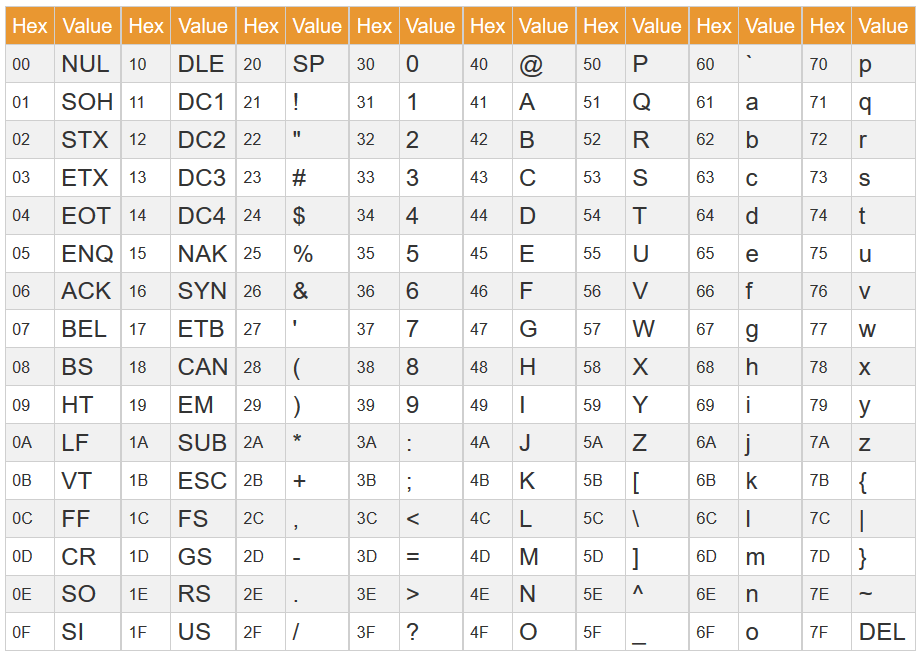
\includegraphics[width=\paperwidth]{ascii_chart_2}
		};
	\end{tikzpicture}
\end{frame}
}

\begin{frame}{ASCII}
	\begin{itemize}
		\pause\item ASCII works OK for English
		\pause\item Standards exist to add another 128 characters (taking us to 8 bits per character)
		\pause\item E.g.\ accented characters for European languages, other Western alphabets e.g. Greek, Cyrillic,
		    mathematical symbols
		\pause\item However 256 characters isn't enough...
	\end{itemize}
\end{frame}

\begin{frame}{Unicode}
	\begin{itemize}
		\pause\item Standard character set developed from 1987 to present day
		\pause\item Currently defines 144697 characters (Unicode 14.0)
		\pause\item First 128 characters are the same as ASCII
		\pause\item Covers most of the world's writing systems
		\pause\item Also covers mathematical symbols and emoji
	\end{itemize}
\end{frame}

\begin{frame}{Encoding Unicode}
    \begin{itemize}
		\pause\item \textbf{UTF-32} encodes characters as 32-bit integers
		\pause\item \textbf{UTF-8} encodes characters as 8, 16, 24 or 32-bit integers
			\begin{itemize}
			    \pause\item 8-bit characters correspond to the first 128 ASCII characters
			        $\implies$ backwards compatible
				\pause\item More common Unicode characters are smaller
				    $\implies$ more efficient than UTF-32
			\end{itemize}
	\end{itemize}
\end{frame}

% \begin{frame}{String representation}
% 	\begin{itemize}
% 		\pause\item \lstinline{"Hello world!"} in ASCII or UTF-8 encoding:
% 	\end{itemize}
	
% 	{\footnotesize\pause\begin{tabular}{*{13}{|c}|}
% 		\hline
% 		72 & 101 & 108 & 108 & 111 & 32 & 119 & 111 & 114 & 108 & 100 & 33 & 0 \\\hline
% 	\end{tabular}}
% \end{frame}

\begin{frame}{UTF-8 representation}
	\begin{itemize}
		\pause\item For characters in ASCII, UTF-8 is the same:
			\begin{itemize}
				\pause\item a $\to [97]$
			\end{itemize}
		\pause\item Other characters are encoded as multi-byte sequences:
			\begin{itemize}
				\pause\item \"u $\to [195, 188]$
				\pause\item 
\includegraphics[height=1.5ex]{chinese}\ $\to [229, 150, 130]$
				\pause\item 
\includegraphics[height=1.5ex]{emoji}\ $\to [240, 159, 152, 130]$
			\end{itemize}
		\pause\item \texttt{"Haha 
\includegraphics[height=1.5ex]{emoji}"} encoded in UTF-8:
	\end{itemize}
	{\footnotesize\pause\begin{tabular}{*{13}{|c}|}
		\hline
		H & a & h & a & space & \multicolumn{4}{c|}{
\includegraphics[height=1.5ex]{emoji}} & null \\\hline
		72 & 97 & 104 & 97 & 32 & 240 & 159 & 152 & 130 & 0 \\\hline
	\end{tabular}}
\end{frame}

% \begin{frame}{Strings in Python}
%     \begin{itemize}
%         \pause\item Python 2 had separate types for ASCII and Unicode strings: \lstinline{str} and \lstinline{unicode}
%         \pause\item Python 3 has just the \lstinline{str} type, which uses Unicode
%         \pause\item String literals are wrapped in \lstinline{'single quotes'} or \lstinline{"double quotes"}
%             (there is no difference)
%     \end{itemize}
% \end{frame}

\begin{frame}[fragile]{Escape sequences}
    \begin{itemize}
        \pause\item Backslash \textbackslash\ has a special meaning in string literals
            --- it denotes the start of an \textbf{escape sequence}
        \pause\item Typically used to write \textbf{non-printable characters}
        \pause\item Most useful: \lstinline{"\n"} is a new line
        \pause\item How to type a backslash character? Use \lstinline{"\\"}
    \end{itemize}
\end{frame}

% \begin{frame}{String literal tricks in Python}
%     \begin{itemize}
%         \pause\item Use triple quotes \lstinline{'''} or \lstinline{"""} for a multi-line string
%         \pause\item Use \lstinline{r" "} or \lstinline{r' '} to turn off escape characters
%             (useful for strings with lots of backslashes, e.g.\ Windows file paths, regular expressions)
%     \end{itemize}
% \end{frame}

\begin{frame}[fragile]{Text files}
    \begin{itemize}
        \pause\item Stored on disk as essentially one long string
        \pause\item Line endings are denoted by non-printable characters
            \begin{itemize}
                \pause\item Unix format: line feed character (ASCII/UTF-8 character 10, \lstinline{"\n"})
                \pause\item Windows format: carriage return character (ASCII/UTF-8 character 13) followed by line feed, \lstinline{"\r\n"}
                \pause\item Most text editors can handle and convert both formats
                \pause\item Most languages allow files to be opened in ``text mode'' which automatically converts
            \end{itemize}
    \end{itemize}
\end{frame}


\part{Other types}
\frame{\partpage}

\begin{frame}{Booleans}
	\begin{itemize}
		\pause\item A \textbf{boolean} can have one of two values: \textbf{true} or \textbf{false}
		\pause\item Python type: \lstinline{bool}
		\pause\item In Python, we have the keywords \lstinline{True} and \lstinline{False}
		\pause\item Could be represented by a single bit in memory...
		\pause\item ... but since memory is addressed in bytes (or words of multiple bytes),
			usually represented as an \lstinline{int} with $0$ meaning \lstinline{False}
			and any non-zero (e.g.\ $1$) meaning \lstinline{True}
	\end{itemize}
\end{frame}

\begin{frame}[fragile]{Boolean values}
	\begin{itemize}
		\pause\item The \lstinline{if} statement takes a boolean value as its condition:
	\end{itemize}
	\begin{lstlisting}
if x > 10:
    print(x)
	\end{lstlisting}
	\begin{itemize}
		\pause\item Variables can also store boolean values:
	\end{itemize}
	\begin{lstlisting}
result = (x > 10)   # result now stores True or False
if result:
    print(x)
	\end{lstlisting}
\end{frame}

\begin{frame}{The ``None'' value}
	\begin{itemize}
		\pause\item Python has a special value \lstinline{None} which can be used to denote the ``absence'' of any other value
		\pause\item Python type: \lstinline{NoneType}
	\end{itemize}
\end{frame}

\begin{frame}[fragile]{Checking types in Python}
	\begin{itemize}
		\pause\item Call \lstinline{type()} to check the type of a variable or value
		\pause\item Note that \lstinline{type()} returns a value of type \lstinline{type}
		\pause\item You can use these \lstinline{type} values like any other value, e.g.
	\end{itemize}
	\begin{lstlisting}
	    if type(x) == int:
	        print("x has type int")
	    elif type(x) == type(y):
	        print("x and y have the same type")
	\end{lstlisting}
\end{frame}

\begin{frame}{Other types}
	\begin{itemize}
		\pause\item \textbf{Container} types for collecting several values
			\begin{itemize}
				\pause\item \lstinline{list}, \lstinline{tuple}, \lstinline{dict}, \lstinline{set}, ...
			\end{itemize}
		\pause\item \textbf{Objects} --- a way to define your own types
		\pause\item Almost everything in Python is a value with a type
			\begin{itemize}
				\pause\item Functions, modules, classes, exceptions, ...
			\end{itemize}
	\end{itemize}
\end{frame}


%\part{Converting types}
\frame{\partpage}

\begin{frame}{Weak vs strong typing}
	\begin{itemize}
		\pause\item In \textbf{weakly typed} languages, a variable can hold a value of any type
        	\begin{itemize}
        	    \pause\item Examples: Python, JavaScript
        	\end{itemize}
		\pause\item In \textbf{strongly typed} languages, the type of a variable must be \textbf{declared}
        	\begin{itemize}
        	    \pause\item Examples: C\#, C++, Java
        	\end{itemize}
	\end{itemize}
\end{frame}

\begin{frame}[fragile]{Weak typing (example in Python)}
    \begin{lstlisting}
x = 7
# Now x has type int

x = "hello"
# Now x has type string
    \end{lstlisting}
\end{frame}

\begin{frame}[fragile]{Strong typing (example in C\#)}
    \begin{lstlisting}[language=C]
int x = 7;
// x is declared with type int

x = "hello";
// Compile error: cannot convert type "string" to "int"
    \end{lstlisting}
\end{frame}

\begin{frame}{Type casting}
	\begin{itemize}
		\pause\item It is often useful to \textbf{cast}, or \textbf{convert}, a value from one type to another
		\pause\item In Python, this is done by calling the type as if it were a function
			\begin{itemize}
				\pause\item \lstinline{float(17)} $\to$ \lstinline{17.0}
				\pause\item \lstinline{int(3.14)} $\to$ \lstinline{3}
				\pause\item \lstinline{str(3.14)} $\to$ \lstinline{"3.14"}
				\pause\item \lstinline{str(1 + 1 == 2)} $\to$ \lstinline{"True"}
				\pause\item \lstinline{int("123")} $\to$ \lstinline{123}
				\pause\item \lstinline{int("five")} gives an error
			\end{itemize}
	\end{itemize}
\end{frame}

\begin{frame}{Operations on types}
	\begin{itemize}
		\pause\item Certain operations can only be done on certain types of values
		\pause\item Can add two ints: \lstinline{2 + 3} $\to$ \lstinline{5}
		\pause\item Can add int and float: \lstinline{2 + 3.1} $\to$ \lstinline{5.1}
		\pause\item Can add two strings: \lstinline{"COMP" + "110"} $\to$ \lstinline{"COMP110"}
		\pause\item Can't add string and int: \lstinline{"COMP" + 110} $\to$ error
	\end{itemize}
\end{frame}

\begin{frame}{Implicit type conversion}
	\begin{itemize}
		\pause\item The type casts we saw a few slides ago are \textbf{explicit}
		\pause\item Some languages (not Python) can perform \textbf{implicit} type casts to make operations work
		\pause\item Sometimes called \textbf{type coercion}
		\pause\item E.g.\ in JavaScript, \lstinline{"COMP" + 110} $\to$ \lstinline{"COMP110"}
		\pause\item The integer \lstinline{110} is implicitly converted to a string \lstinline{"110"} to make the addition work
		\pause\item Equivalent in Python with explicit casts: \lstinline{"COMP" + str(110)}
	\end{itemize}
\end{frame}

\begin{frame}{Dangers of implicit type conversion}
	\begin{itemize}
		\pause\item Rules for implicit type conversion can sometimes be confusing
		\pause\item E.g.\ in JavaScript:
			\begin{itemize}
				\pause\item \lstinline{"5" + 3} $\to$ \lstinline{"53"}
				\pause\item \lstinline{"5" - 3} $\to$ \lstinline{2}
			\end{itemize}
	\end{itemize}
\end{frame}


\part{Logic gates}
\frame{\partpage}

\newcommand{\TT}{\textsc{True}}
\newcommand{\FF}{\textsc{False}}
\newcommand{\OP}[1]{\ \textsc{#1}\ }
\newcommand{\OPand}{\OP{and}}
\newcommand{\OPor}{\OP{or}}
\newcommand{\OPxor}{\OP{xor}}
\newcommand{\OPnand}{\OP{nand}}
\newcommand{\OPnor}{\OP{nor}}
\newcommand{\OPxnor}{\OP{xnor}}
\newcommand{\OPnot}{\textsc{not}\ }

\newcommand{\OPname}{}
\newcommand{\OPenglishA}{}
\newcommand{\OPenglishB}{}
\newcommand{\OPtable}{}
\newcommand{\OPdiagram}{}

\newcommand{\OPframe}[5]{
	\begin{frame}{#1}
		\pause
		\begin{center}
			#2 \par if and only if \par #3
		\end{center}
		\pause
		\begin{columns}
			\begin{column}{0.48\textwidth}
				\begin{center}
					#4
				\end{center}
			\end{column}
			\pause
			\begin{column}{0.48\textwidth}
				\begin{center}
					\begin{circuitikz} \draw[color=\circuitcolour]
						#5
					\end{circuitikz}
				\end{center}
			\end{column}
		\end{columns}
	\end{frame}
}

\begin{frame}{Boolean logic}
	\begin{itemize}
		\pause\item Works with two values: \TT\ and \FF
		\pause\item Foundation of the \textbf{digital computer}:
			represented in circuits as \textbf{on} and \textbf{off}
		\pause\item Representing as $1$ and $0$ leads to \textbf{binary notation}
		\pause\item One boolean value = one \textbf{bit} of information
		\pause\item Programmers use boolean logic for conditions in \lstinline{if} and \lstinline{while}
			statements
	\end{itemize}
\end{frame}

%\begin{frame}{Simulating logic circuits}
	%\centering
	%\url{http://logic.ly/demo/}
%\end{frame}

\OPframe{Not}
	{$\OPnot A$ is \TT}{$A$ is \FF}
	{\begin{tabular}{|c||c|} \hline
		$A$ & $\OPnot A$ \\\hline
		\FF & \TT \\
		\TT & \FF \\\hline
	\end{tabular}}
	{ (0,0) node[not port] (gate) {}
	(gate.in)  node[anchor=east] {$A$}
	(gate.out) node[anchor=west] {$\OPnot A$}
	; }

\OPframe{And}
	{$A \OPand B$ is \TT}{\textbf{both $A$ and $B$} are \TT}
	{\begin{tabular}{|c|c||c|}
		\hline
		$A$ & $B$ & $A \OPand B$ \\\hline
		\FF & \FF & \FF \\
		\FF & \TT & \FF \\
		\TT & \FF & \FF \\
		\TT & \TT & \TT \\\hline
	\end{tabular}}
	{ (0,0) node[and port] (gate) {}
	(gate.in 1) node[anchor=east] {$A$}
	(gate.in 2) node[anchor=east] {$B$}
	(gate.out)  node[anchor=west] {$A \OPand B$}
	; }

\OPframe{Or}
	{$A \OPor B$ is \TT}{\textbf{either $A$ or $B$, or both,} are \TT}
	{\begin{tabular}{|c|c||c|}
		\hline
		$A$ & $B$ & $A \OPand B$ \\\hline
		\FF & \FF & \FF \\
		\FF & \TT & \TT \\
		\TT & \FF & \TT \\
		\TT & \TT & \TT \\\hline
	\end{tabular}}
	{ (0,0) node[or port] (gate) {}
	(gate.in 1) node[anchor=east] {$A$}
	(gate.in 2) node[anchor=east] {$B$}
	(gate.out)  node[anchor=west] {$A \OPor B$}
	; }

\begin{frame}{Socrative \texttt{FALCOMPED}}
	What is the value of
	$$ A \OPand (B \OPor C) $$
	when
	\begin{align*}
		A &= \TT \\
		B &= \FF \\
		C &= \TT
	\end{align*}
	?
\end{frame}

\begin{frame}{Socrative \texttt{FALCOMPED}}
	What is the value of
	$$ (\OPnot A) \OPand (B \OPor C) $$
	when
	\begin{align*}
		A &= \TT \\
		B &= \FF \\
		C &= \TT
	\end{align*}
	?
\end{frame}

\begin{frame}{Socrative \texttt{FALCOMPED}}
	For what values of $A, B, C, D$ is
	$$ A \OPand \OPnot B \OPand \OPnot (C \OPor D) = \TT $$
	?
\end{frame}

\begin{frame}{Socrative \texttt{FALCOMPED}}
	What is the value of
	$$ A \OPor \OPnot A $$
	?
\end{frame}

\begin{frame}{Socrative \texttt{FALCOMPED}}
	What is the value of
	$$ A \OPand \OPnot A $$
	?
\end{frame}

\begin{frame}{Socrative \texttt{FALCOMPED}}
	What is the value of
	$$ A \OPor A $$
	?
\end{frame}

\begin{frame}{Socrative \texttt{FALCOMPED}}
	What is the value of
	$$ A \OPand A $$
	?
\end{frame}

\begin{frame}{Socrative \texttt{FALCOMPED}}
	What expression is equivalent to this circuit?
	\begin{center}
		\begin{circuitikz} \draw[color=\circuitcolour]
			(0,0) node[and port] (gateA) {}
			(0,-2) node[or port] (gateB) {}
			(1,0) node[not port] (gateC) {}
			(3.5,-1) node[or port] (gateD) {}
			(gateA.out) -- (gateC.in) {}
			(gateC.out) -| (gateD.in 1) {}
			(gateB.out) -| (gateD.in 2) {}
			(gateD.out) node[anchor=west] {?}
			(gateA.in 1) node[anchor=east] {$A$}
			(gateA.in 2) node[anchor=east] {$B$}
			(gateB.in 1) node[anchor=east] {$C$}
			(gateB.in 2) node[anchor=east] {$D$}
			;
		\end{circuitikz}
	\end{center}
\end{frame}

\begin{frame}[fragile]{Writing logical operations}
	\pause
	\centering
	\begin{tabular}{|c||c|c|c|}
		\hline
		Operation & Python & C family & Mathematics \\\hline
		$\OPnot A$
			& \texttt{not a}
			& \texttt{!a}
			& $\neg A$ {\huge\phantom{$I$}} or {\huge\phantom{$I$}} $\overline{A}$
			\pause\\
		$A \OPand B$ 
			& \texttt{a and b}
			& \texttt{a \&\& b}
			& $A \wedge B$
			\pause\\
		$A \OPor B$ 
			& \texttt{a or b}
			& \texttt{a || b}
			& $A \vee B$
			\\\hline
	\end{tabular}
	\pause
	\par\vspace{2ex}\par
	Other operators can be expressed by combining these
\end{frame}

\begin{frame}{De Morgan's Laws}
	\pause
	$$ \OPnot (A \OPor B) = (\OPnot A) \OPand (\OPnot B) $$
	\pause
	$$ \OPnot (A \OPand B) = (\OPnot A) \OPor (\OPnot B) $$
	\pause
	Proof: Worksheet 4, questions 3a and 3b
\end{frame}

\part{Truth tables}
\frame{\partpage}

\begin{frame}{Enumeration}
	\begin{itemize}
		\pause\item Since booleans have only two possible values, we can often \textbf{enumerate}
			all possible values of a set of boolean variables
		\pause\item For $n$ variables there are $2^n$ possible combinations
		\pause\item Essentially, all the $n$-bit binary numbers
		\pause\item A \textbf{truth table} enumerates all the possible values of a boolean expression
		\pause\item Can be used to prove that two expressions are equivalent
	\end{itemize}
\end{frame}

\begin{frame}{Truth table example}
	$$ (A \OPor \OPnot B) \OPand C $$
	\begin{centering}
	    \small
		\begin{tabular}{|ccc|cc|c|}
		    \hline
			$A$ & $B$ & $C$ & $\OPnot B$ & $A \OPor \OPnot B$ & $(A \OPor \OPnot B) \OPand C$ \\\hline\pause
			\FF & \FF & \FF & \TT & \TT & \FF \\\pause
			\FF & \FF & \TT & \TT & \TT & \TT \\\pause
			\FF & \TT & \FF & \FF & \FF & \FF \\\pause
			\FF & \TT & \TT & \FF & \FF & \FF \\\pause
			\TT & \FF & \FF & \TT & \TT & \FF \\\pause
			\TT & \FF & \TT & \TT & \TT & \TT \\\pause
			\TT & \TT & \FF & \FF & \TT & \FF \\\pause
			\TT & \TT & \TT & \FF & \TT & \TT \\\hline
		\end{tabular}
	\end{centering}
\end{frame}

\part{Other logic gates}
\frame{\partpage}

\OPframe{Exclusive Or}
	{$A \OPxor B$ is \TT}{\textbf{either $A$ or $B$, but not both,} are \TT}
	{\begin{tabular}{|c|c||c|}
		\hline
		$A$ & $B$ & $A \OPand B$ \\\hline
		\FF & \FF & \FF \\
		\FF & \TT & \TT \\
		\TT & \FF & \TT \\
		\TT & \TT & \FF \\\hline
	\end{tabular}}
	{ (0,0) node[xor port] (gate) {}
	(gate.in 1) node[anchor=east] {$A$}
	(gate.in 2) node[anchor=east] {$B$}
	(gate.out)  node[anchor=west] {$A \OPxor B$}
	; }

\begin{frame}{Socrative \texttt{FALCOMPED}}
	How can $A \OPxor B$ be written using the operations $\OPand, \OPor, \OPnot$?
\end{frame}

\begin{frame}
    \begin{center}
        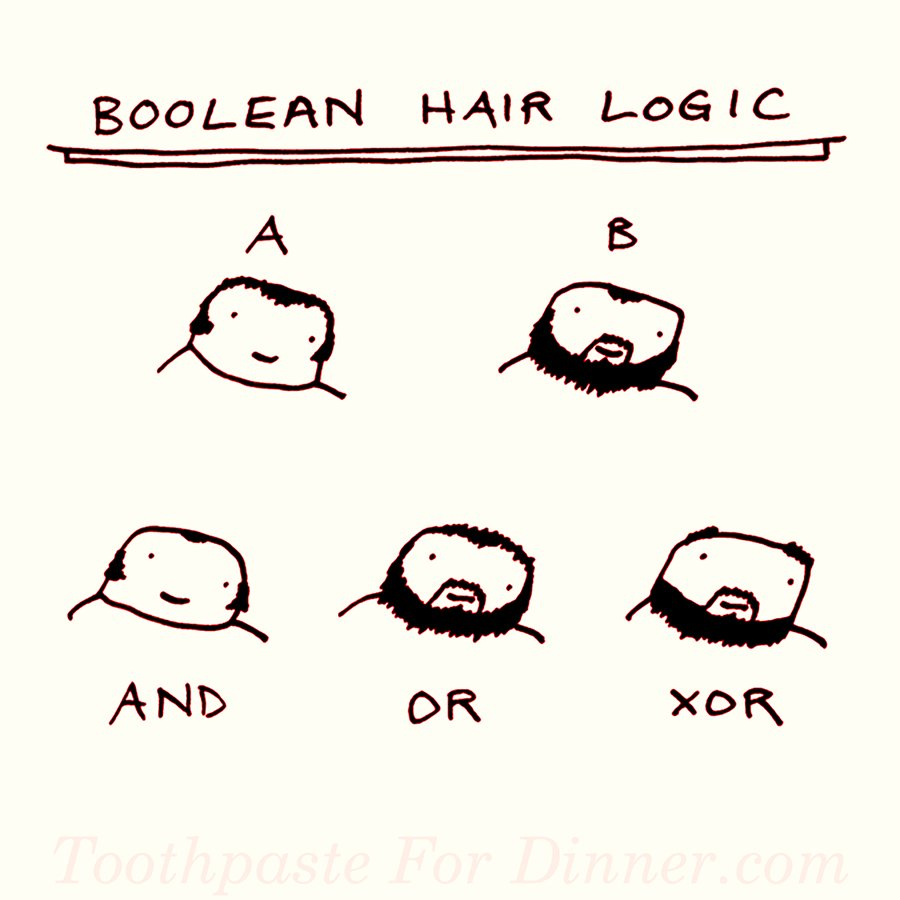
\includegraphics[width=0.8\textwidth]{boolean_hair_logic}
    \end{center}
\end{frame}

\begin{frame}{Negative gates}
	\pause
	\begin{center}
		$\OPnand, \OPnor, \OPxnor$ \par are the \textbf{negations} of \par $\OPand, \OPor, \OPxor$
	\end{center}
	\pause
	\begin{columns}
		\begin{column}{0.48\textwidth}
			\begin{center}
				\begin{align*}
					A \OPnand B &= \OPnot (A \OPand B) \\
					A \OPnor B &= \OPnot (A \OPor B) \\
					A \OPxnor B &= \OPnot (A \OPxor B)
				\end{align*}
			\end{center}
		\end{column}
		\pause
		\begin{column}{0.48\textwidth}
			\begin{center}
				\begin{circuitikz} \draw[color=\circuitcolour]
					(0,0) node[nand port] (gate) {}
					(gate.in 1) node[anchor=east] {$A$}
					(gate.in 2) node[anchor=east] {$B$}
					(gate.out)  node[anchor=west] {$A \OPnand B$}
					;
				\end{circuitikz}
				\begin{circuitikz} \draw[color=\circuitcolour]
					(0,0) node[nor port] (gate) {}
					(gate.in 1) node[anchor=east] {$A$}
					(gate.in 2) node[anchor=east] {$B$}
					(gate.out)  node[anchor=west] {$A \OPnor B$}
					;
				\end{circuitikz}
				\begin{circuitikz} \draw[color=\circuitcolour]
					(0,0) node[xnor port] (gate) {}
					(gate.in 1) node[anchor=east] {$A$}
					(gate.in 2) node[anchor=east] {$B$}
					(gate.out)  node[anchor=west] {$A \OPxnor B$}
					;
				\end{circuitikz}
			\end{center}
		\end{column}
	\end{columns}
\end{frame}

\begin{frame}{Any logic gate can be constructed from NAND gates}
    \begin{center}
        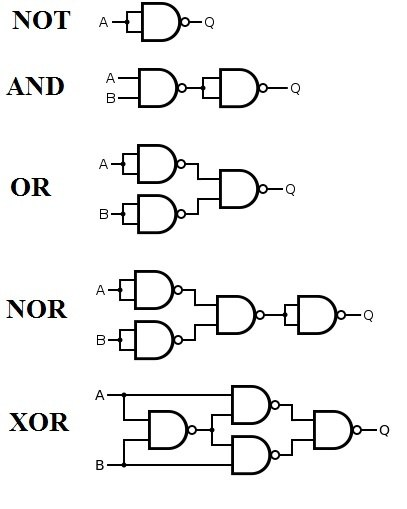
\includegraphics[height=0.7\textheight]{nand_gates}
    \end{center}
\end{frame}

\begin{frame}{What does this circuit do?}
	\centering
	\begin{circuitikz} \draw[color=\circuitcolour]
		(0,0) node[nand port] (gateA) {}
		(0,-2) node[nand port] (gateB) {}
		(gateA.out) -- ($ (gateA.out) + (0, -0.5) $) -- ($ (gateB.in 1) + (0, 0.5) $) -- (gateB.in 1) {}
		(gateB.out) -- ($ (gateB.out) + (0, 0.5) $) -- ($ (gateA.in 2) + (0, -0.5) $) -- (gateA.in 2) {}
		(gateA.out) -- ($ (gateA.out) + (0.5, 0) $) node[anchor=west] {$Q$}
		(gateB.out) -- ($ (gateB.out) + (0.5, 0) $) node[anchor=west] {$\overline{Q}$}
		(gateA.in 1) -- ($ (gateA.in 1) + (-0.5, 0) $) node[anchor=east] {$S$}
		(gateB.in 2) -- ($ (gateB.in 2) + (-0.5, 0) $) node[anchor=east] {$R$}
		;
	\end{circuitikz}
	\begin{itemize}
		\pause\item This is called a \textbf{NAND latch}
		\pause\item It ``remembers'' a single boolean value
		\pause\item Put a few billion of these together
			(along with some control circuitry)
			and you've got \textbf{memory}!
	\end{itemize}
\end{frame}

\begin{frame}{NAND gates}
    \begin{itemize}
        \pause\item All arithmetic and logic operations, as well as memory, can be built from NAND gates
        \pause\item So an entire computer can be built just from NAND gates!
        \pause\item Play the game: \url{http://nandgame.com}
        \pause\item NAND gate circuits are \textbf{Turing complete}
        \pause\item The same is true of NOR gates
    \end{itemize}
\end{frame}



\end{document}
